\documentclass{beamer}
\usetheme[progressbar=frametitle]{metropolis}          % Use metropolis theme

\graphicspath{{../src/images/}}

\usepackage{longtable}
\usepackage{pdfpages}	


\newcommand{\SubItem}[1]{
    {\setlength\itemindent{15pt} \item[]#1}
}


% change progressbar thickness
\makeatletter
\setlength{\metropolis@titleseparator@linewidth}{1.5pt}
\setlength{\metropolis@progressonsectionpage@linewidth}{1.5pt}
\setlength{\metropolis@progressinheadfoot@linewidth}{2pt}
\makeatother

\usepackage{FiraSans}
\usepackage{makecell}
\usepackage{appendixnumberbeamer}

\title{Bezdrátová senzorová síť pro přístupový systém}
\date{25.6.2020}
\author{Bc. Tomáš Hyhlík \\
Vedoucí: Ing. Bc. Marek Neruda, Ph.D}
\institute{Katedra Mikroelektroniky}
\begin{document}
	\maketitle
  



%%%%%%%%%%%%%%%%%%%%%%%%%%%%
\begin{frame}{Integrace WSN do architektury přístupového systému}

	\begin{itemize}
		\item Projek ve firme IMA s.r.o.
		\item Spolufinancovano z dotace od SGS a.s.

		\item Vytvoren clanek pro odborny casopis:
		\SubItem 	- Advances in Electrical and Electronic Engineering
		\SubItem 	- http://advances.utc.sk/index.php/AEEE
		\SubItem 	- Indexován v databázi WoS a Scopus.

	\end{itemize}

\end{frame}

	

%%%%%%%%%%%%%%%%%%%%%%%%%%%%
\begin{frame}{Integrace WSN do architektury přístupového systému}

	\begin{figure}[h]
		\centering
		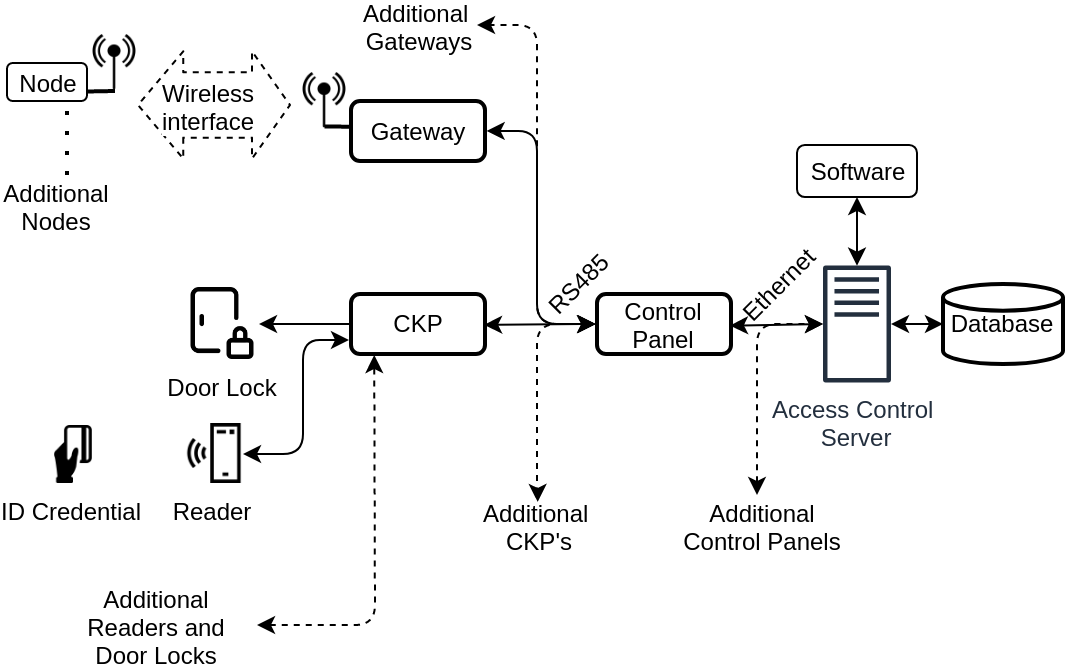
\includegraphics[width=1\textwidth]{ACS_IoT_extension_21}
		% \caption{Architektura přístupového systému firmy IMA s rozšířením o gateway senzorové sítě}
		\label{fig:ACS architecture IMA with geteway}
	\end{figure}
		
\end{frame}



%%%%%%%%%%%%%%%%%%%%%%%%%%%%
\begin{frame}{Výběr bezdrátové technologie pro senzorovou síť}
	Požadavky:
	\begin{itemize}
		\item Nízká cena HW
		\item Jednoduché připojení koncových zařízení třetích stran (Third party)
		\item Velký počet dostupných koncových zařízení třetích stran na trhu 
		\item Jednoduchá implementace sítě
		\item Nízká spotřeba energie koncových zařízení
	\end{itemize}

\end{frame}


%%%%%%%%%%%%%%%%%%%%%%%%%%%%
\begin{frame} {WSN gateway - HW}
	\begin{figure}[!h]
		\centering
		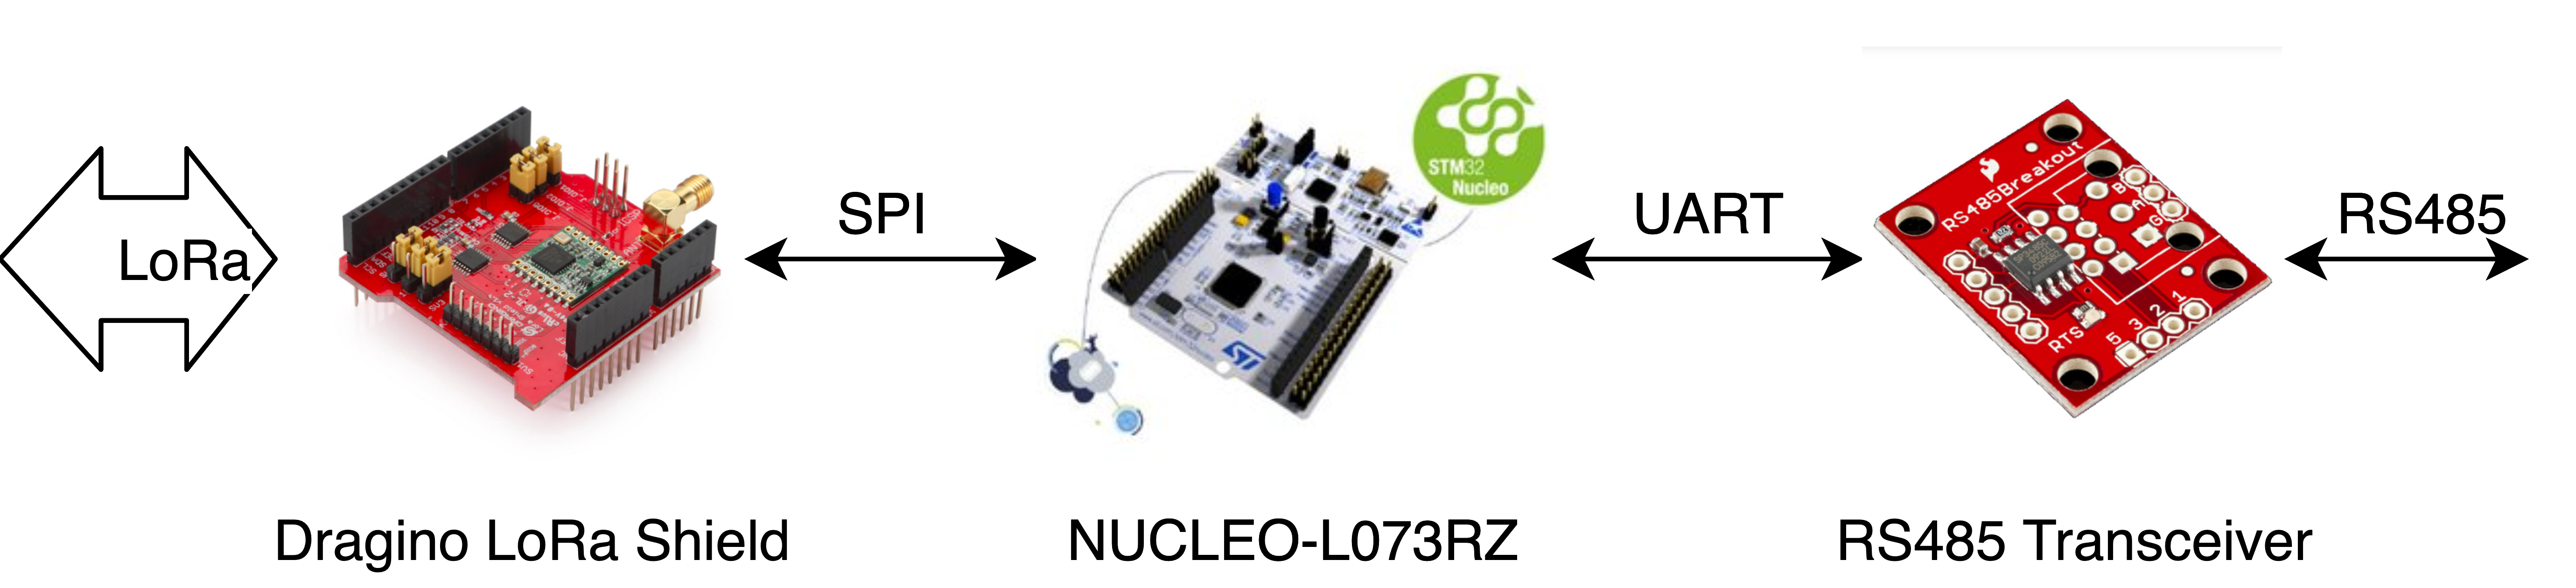
\includegraphics[width=1\textwidth]{LoRaWAN_gw_RS485_blockDiagram_3}
		% \caption{Blokový diagram navržené gatewaye senzorové sítě, Dragino LoRa Shield \cite{draginoWiki}, RS485 transceiver \cite{rs485tr}, NUCLEO-L073RZ \cite{nucleo-l073RZ_ST}}
		\label{fig:gatewayBlockDiagram}
	\end{figure}

	Blokový diagram navržené gatewaye senzorové sítě, Dragino LoRa Shield \cite{draginoWiki}, RS485 transceiver \cite{rs485tr}, NUCLEO-L073RZ \cite{nucleo-l073RZ_ST}

\end{frame}

%%%%%%%%%%%%%%%%%%%%%%%%%%%%
\begin{frame} {WSN gateway - vývoj SW}
	% {\fontsize{9}{5}\selectfont 
		Rozdělení SW na nezávislé moduly:
		\begin{itemize}
			\item LoRa
			\item LoRaWAN\_packet
			\item LoRa\_sensors
			\item rs485\_protocol
			\item usb
			\item eeprom
		\end{itemize}

		Doplňkové knihovny:
		\begin{itemize}
			\item buffer\_ring
			\item ByteArray
			\item LinkedList\_ByteArray
			\item aes (tiny-aes) \cite{lib_tiny-AES128-C} 
			\item cmac (openpana) \cite{lib_openpana}
		\end{itemize}
	% }
\end{frame}



%%%%%%%%%%%%%%%%%%%%%%%%%%%%
\begin{frame} {Testování navržené gatewaye}
	Za běžném provozu
	V budově FEL, blok A4, 5. patro

	Připojená zařízení v testované síti RS485
	\begin{itemize}
		\item 1 kontrolní panel
		\item 12 CKP zařízení (páry čteček a dveřních zámků)
		\item 1 gateway senzorové sítě + 2 senzory
	\end{itemize}

	\begin{figure}[!h]
		\centering
		\includegraphics[width=1\textwidth]{5patro}
	\end{figure}

\end{frame}


%%%%%%%%%%%%%%%%%%%%%%%%%%%%
\begin{frame} {Výpočet maximálního počtu koncových zařízení senzorové sítě}

	od 21. září do 31. října

	\begin{figure}[!h]
		\centering
		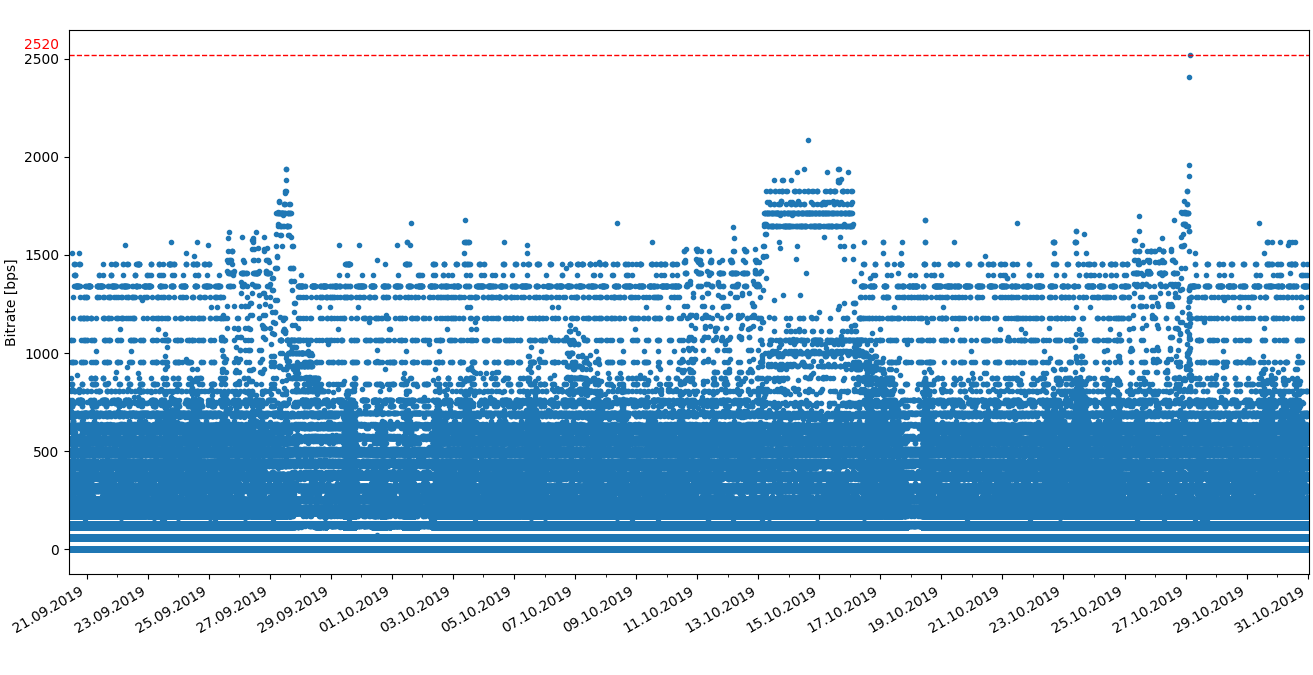
\includegraphics[width=1\textwidth]{03-dr-measured}
	\end{figure}





	
\end{frame}


%%%%%%%%%%%%%%%%%%%%%%%%%%%%
\begin{frame} {Výpočet maximálního počtu koncových zařízení senzorové sítě}

	\vspace{-12pt}

	\begin{equation}
		S_{MAX} = \frac{\frac{\frac{v_{485}}{B}}{l_{MAX}} - R}{P}
		% \label{equ:max-count-of-sensors}
		\end{equation}
		
	\fontsize{10}{12}\selectfont 

	% 	kde:
		
	% 	\begin{tabular}{l @{  } l}
	% 	$v_{485}$ & rychlost přenosu dat v síti RS485 [bps]\\
	% 	B        & počet bitů v bytu (pro přepočítání rychlosti přenosu dat na byty) \\
	% 	$l_{MAX}$ & maximální délka paketu \\
	% 	R        & rezerva rychlosti přenosu dat [\%]\\
	% 	P        & počet paketů k přenesení dat z koncového zařízení \\
	% \end{tabular}


	\begin{longtable} {|l|llll|}
		% % \footnotesize
		% \caption{Maximální počet připojených koncových zařízení v senzorové síti souběžně odesílající data skrze síť RS485 s určitou    
		% 	rezervou}      \label{tab:max-sensor-nodes} \\
			\hline
			\textbf{RS485 rychlost přenosu dat} &       \multicolumn{4}{c|}{\textbf{Rezerva R}}	  	    \\
			$v_{485}$ {[bps]}  &	0 \%	&	10 \%	&	20 \%	&	30 \%  \\ \hline
		
			1200~~~ &    1	&    1	&    1	&    1 \\
			2400~~~ &    3	&    3	&    3	&    2 \\
			4800~~~ &    7	&    6	&    6	&    5 \\
			9600~~~ &   15	&   13	&   12	&   10 \\
			19200~~~ &   30	&   27	&   24	&   21 \\
			38400~~~ &   60	&   54	&   48	&   42 \\
			57600~~~ &   90	&   81	&   72	&   63 \\
			115200~~~ &  180	&  162	&  144	&  126 \\
			230400~~~ &  360	&  324	&  288	&  252 \\
			460800~~~ &  720	&  648	&  576	&  504 \\
			921600~~~ & 1440	& 1296	& 1152	& 1008 \\
			\hline
		
		\end{longtable}
\end{frame}


%%%%%%%%%%%%%%%%%%%%%%%%%%%%
\begin{frame}{Vylepšení prototypu navržené gatewaye - schéma}
	\begin{figure}[!h]
		\centering
		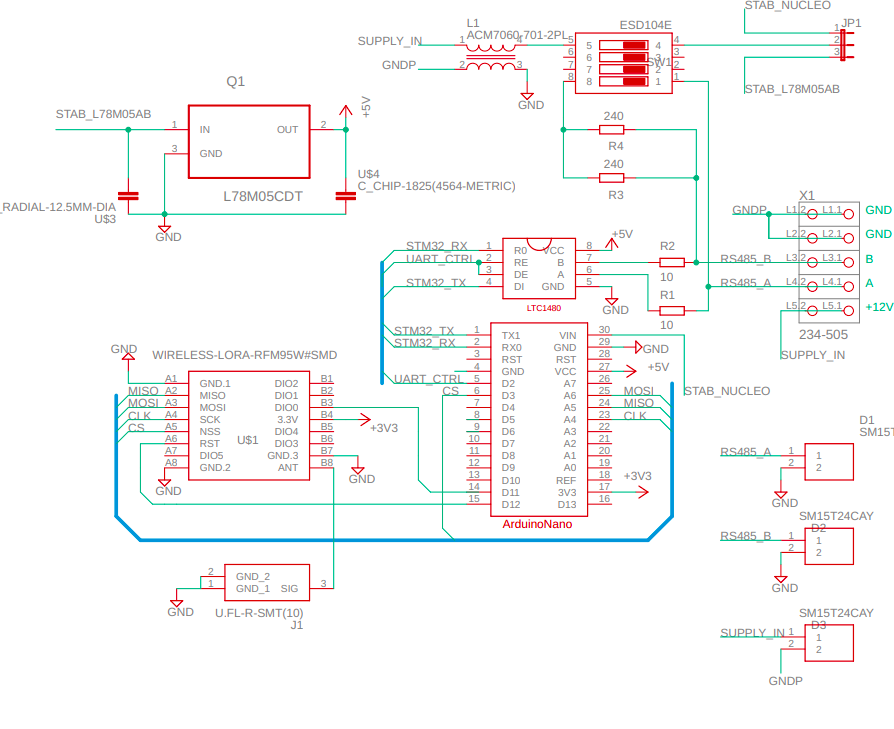
\includegraphics[width=1\textwidth]{minigateway_schema}
		\caption{Návrh gatewaye verze 2 - schéma}
		\label{fig:minigateway_schema}
	\end{figure}
\end{frame}


%%%%%%%%%%%%%%%%%%%%%%%%%%%%
\begin{frame}{Vylepšení prototypu navržené gatewaye - foto}
	\begin{figure}[!h]
		\centering
		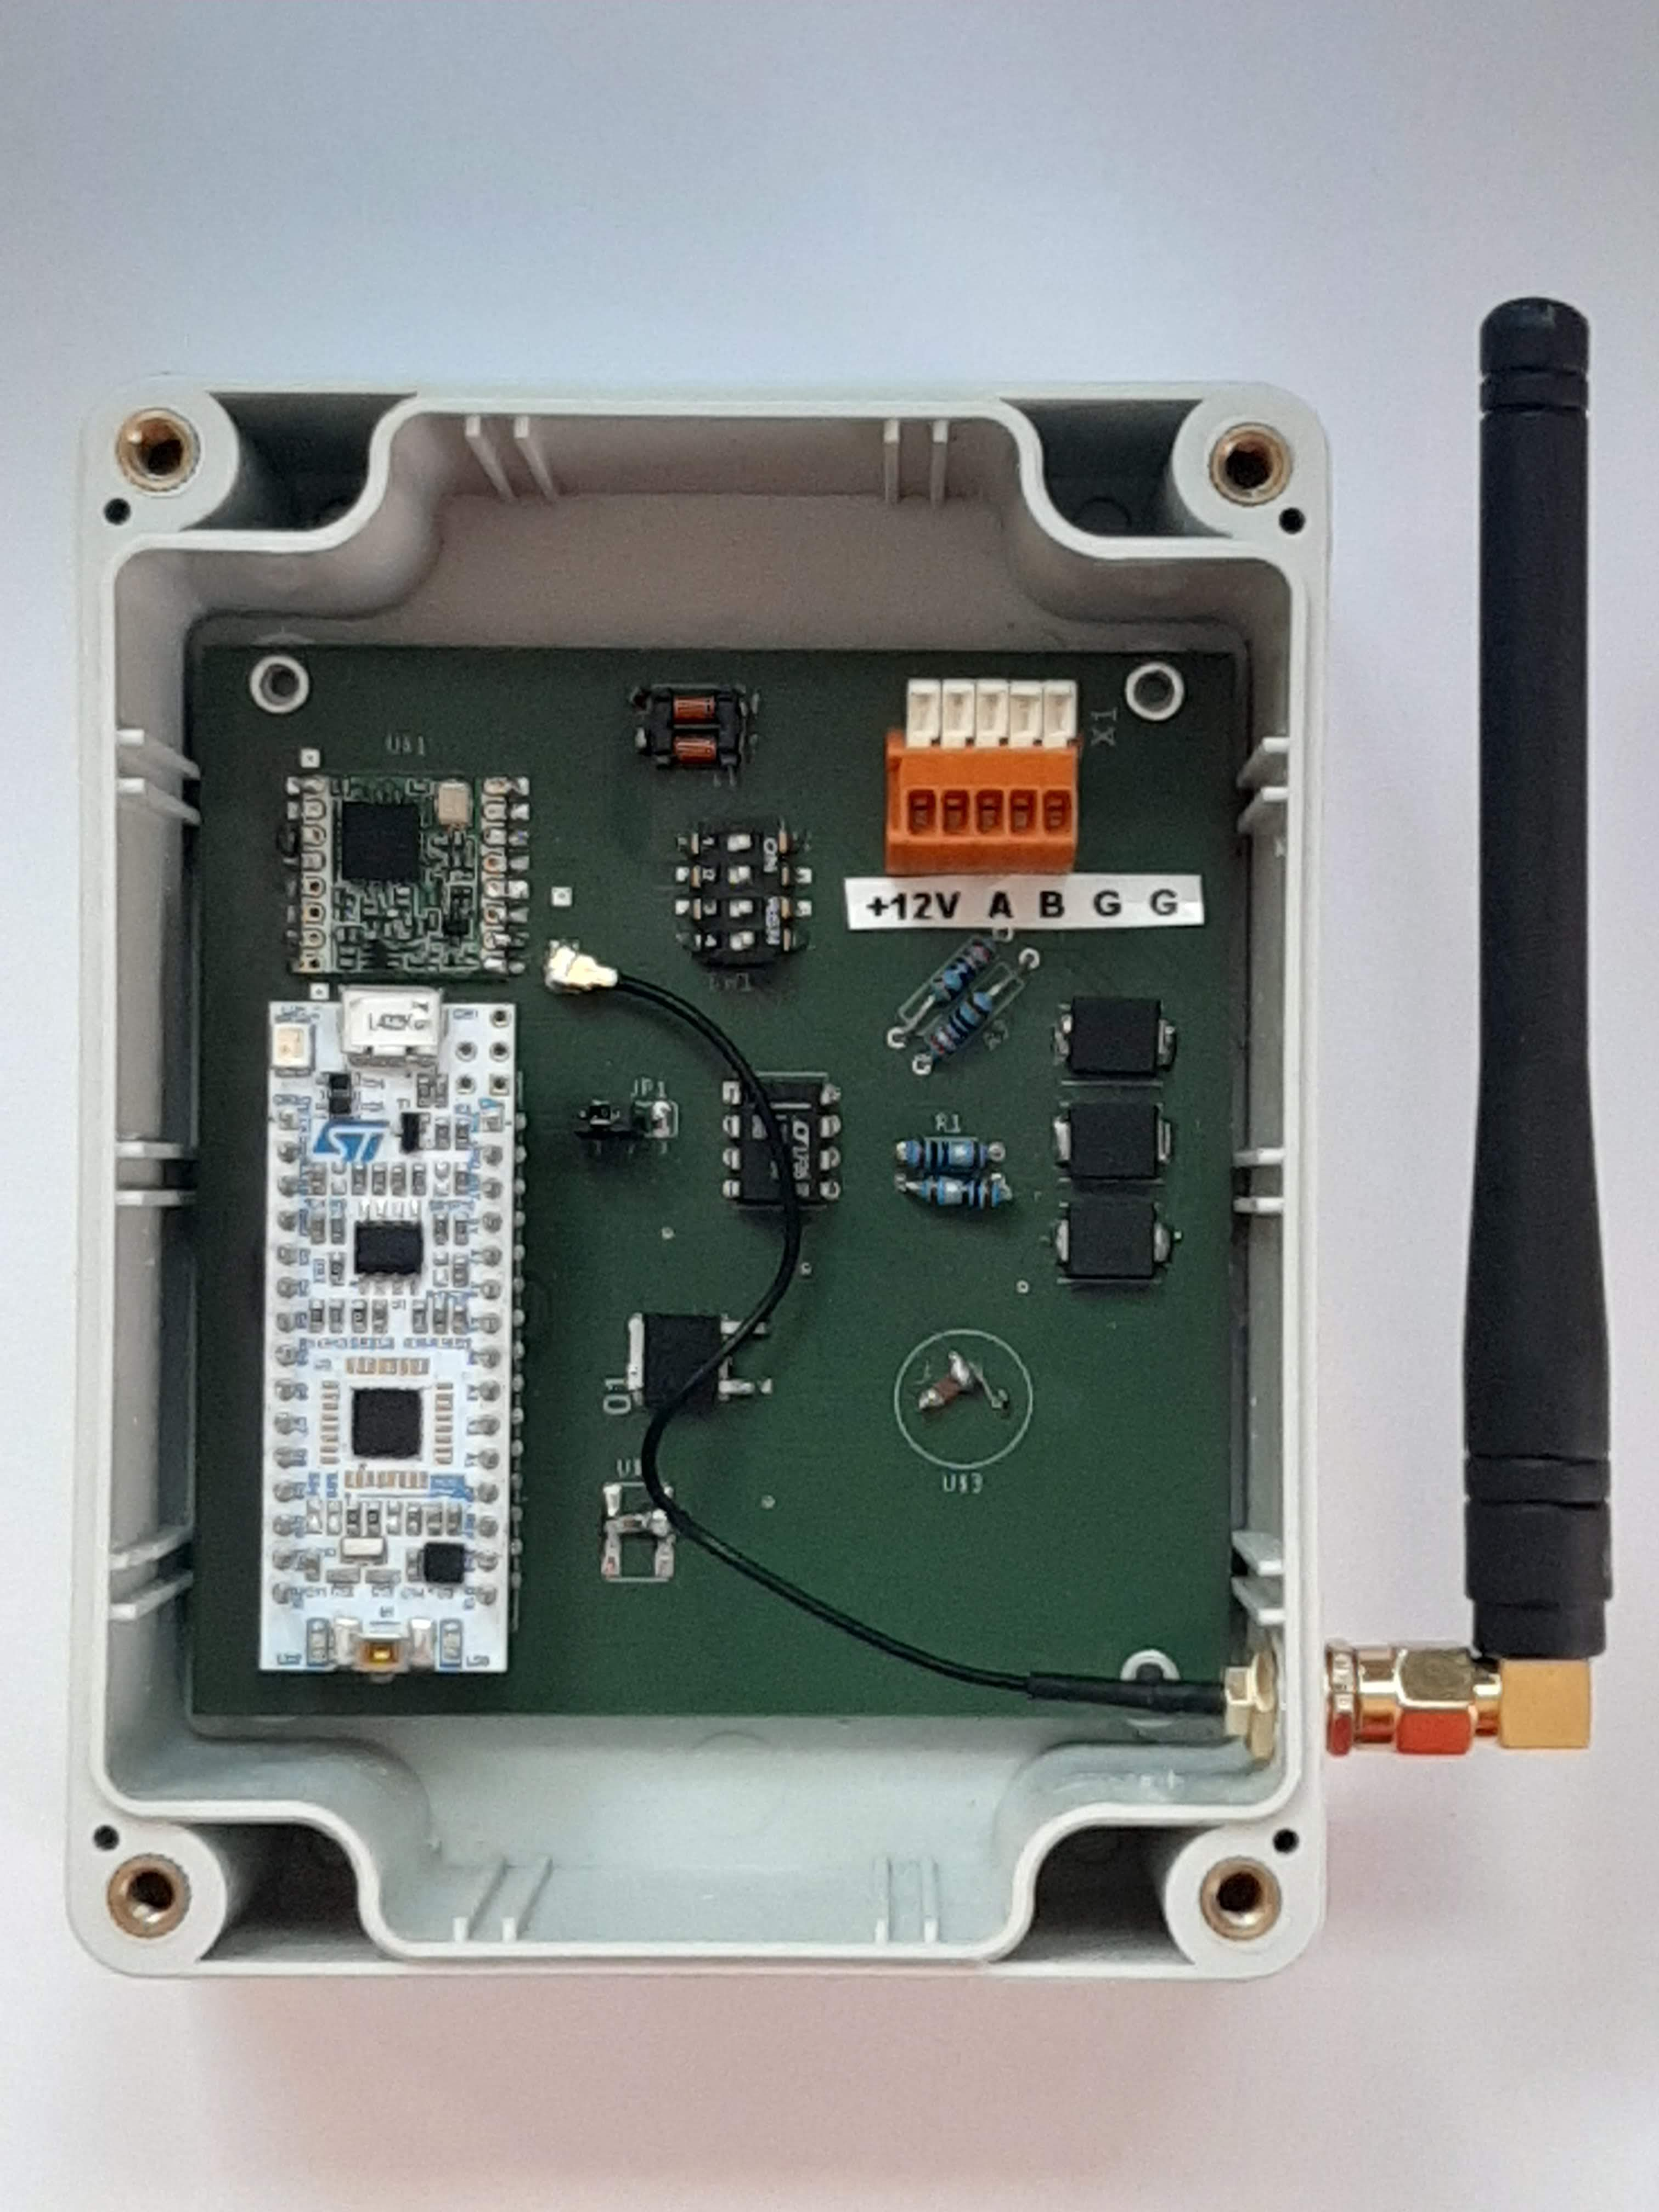
\includegraphics[width=0.6\textwidth]{photo_minigatewayV2}
		\caption{Foto gatewaye verze 2}
		\label{fig:minigateway_fotoV2}
	\end{figure}
\end{frame}


%%%%%%%%%%%%%%%%%%%%%%%%%%%%
\begin{frame}{}
	\section{Děkuji za pozornost}
\end{frame}


%%%%%%%%%%%%%%%%%%%%%%%%%%%%
\begin{frame}{Otázky vedoucího}
		\textbf{Co znamená pojem orientace komunikace? Str. 11}
		\\
		\hspace{10pt}
		Nekorektnost. Místo orientace komunikace má být směr posílání dat.
		\vspace{15pt}		

		\textbf{Zhodnoťte správnost odhadu max. počtu připo
		jených koncových zařízení z testování provozu v síti RS 485. Kapitola 5.}
		\\
		\hspace{10pt}
		Nekorektnost. Nejedná se o odhad, ale o výpočet.
		\vspace{15pt}		

\end{frame}

%%%%%%%%%%%%%%%%%%%%%%%%%%%%
\begin{frame}{Otázky oponenta}
		\textbf{Jak je chráňeno rozhraní RS485 u vyvinuté gatewaye před přepětím}
		\\
		\hspace{10pt}
		Transil typu SM15T15CA s průrazným napětím 15 V, spojující linky A a B ke GND.
		
\end{frame}



	% \begin{itemize}
	% 	\item 	Co znamená pojem orientace komunikace? Str. 11
	% 	\item 	Zhodnoťte správnost odhadu max. počtu připojených koncových zařízení z testování provozu v síti RS 485. Kapitola 5.
	% 	\item Jak je chráňeno rozhraní RS485 u vyvinuté gatewaye před přepětím
	% \end{itemize}





%%%%%%%%%%%%%%%%%%%%%%%%%%%%

\frame[allowframebreaks]{  

	\section{References}

	\bibliographystyle{apalike}
	\bibliography{Biblio-Database}

}








\end{document}